\documentclass[journal,12pt,twocolumn]{IEEEtran}

\usepackage{setspace}
\usepackage{gensymb}
\singlespacing
\usepackage[cmex10]{amsmath}

\usepackage{amsthm}

\usepackage{mathrsfs}
\usepackage{txfonts}
\usepackage{stfloats}
\usepackage{bm}
\usepackage{cite}
\usepackage{cases}
\usepackage{subfig}

\usepackage{longtable}
\usepackage{multirow}

\usepackage{enumitem}
\usepackage{mathtools}
\usepackage{steinmetz}
\usepackage{tikz}
\usepackage{circuitikz}
\usepackage{verbatim}
\usepackage{tfrupee}
\usepackage[breaklinks=true]{hyperref}
\usepackage{graphicx}
\usepackage{tkz-euclide}

\usetikzlibrary{calc,math}
\usepackage{listings}
    \usepackage{color}                                            %%
    \usepackage{array}                                            %%
    \usepackage{longtable}                                        %%
    \usepackage{calc}                                             %%
    \usepackage{multirow}                                         %%
    \usepackage{hhline}                                           %%
    \usepackage{ifthen}                                           %%
    \usepackage{lscape}     
\usepackage{multicol}
\usepackage{chngcntr}

\DeclareMathOperator*{\Res}{Res}

\renewcommand\thesection{\arabic{section}}
\renewcommand\thesubsection{\thesection.\arabic{subsection}}
\renewcommand\thesubsubsection{\thesubsection.\arabic{subsubsection}}

\renewcommand\thesectiondis{\arabic{section}}
\renewcommand\thesubsectiondis{\thesectiondis.\arabic{subsection}}
\renewcommand\thesubsubsectiondis{\thesubsectiondis.\arabic{subsubsection}}


\hyphenation{op-tical net-works semi-conduc-tor}
\def\inputGnumericTable{}                                 %%

\lstset{
%language=C,
frame=single, 
breaklines=true,
columns=fullflexible
}
\begin{document}


\newtheorem{theorem}{Theorem}[section]
\newtheorem{problem}{Problem}
\newtheorem{proposition}{Proposition}[section]
\newtheorem{lemma}{Lemma}[section]
\newtheorem{corollary}[theorem]{Corollary}
\newtheorem{example}{Example}[section]
\newtheorem{definition}[problem]{Definition}

\newcommand{\BEQA}{\begin{eqnarray}}
\newcommand{\EEQA}{\end{eqnarray}}
\newcommand{\define}{\stackrel{\triangle}{=}}
\bibliographystyle{IEEEtran}
\raggedbottom
\setlength{\parindent}{0pt}
\providecommand{\mbf}{\mathbf}
\providecommand{\pr}[1]{\ensuremath{\Pr\left(#1\right)}}
\providecommand{\qfunc}[1]{\ensuremath{Q\left(#1\right)}}
\providecommand{\sbrak}[1]{\ensuremath{{}\left[#1\right]}}
\providecommand{\lsbrak}[1]{\ensuremath{{}\left[#1\right.}}
\providecommand{\rsbrak}[1]{\ensuremath{{}\left.#1\right]}}
\providecommand{\brak}[1]{\ensuremath{\left(#1\right)}}
\providecommand{\lbrak}[1]{\ensuremath{\left(#1\right.}}
\providecommand{\rbrak}[1]{\ensuremath{\left.#1\right)}}
\providecommand{\cbrak}[1]{\ensuremath{\left\{#1\right\}}}
\providecommand{\lcbrak}[1]{\ensuremath{\left\{#1\right.}}
\providecommand{\rcbrak}[1]{\ensuremath{\left.#1\right\}}}
\theoremstyle{remark}
\newtheorem{rem}{Remark}
\newcommand{\sgn}{\mathop{\mathrm{sgn}}}
\providecommand{\abs}[1]{\left\vert#1\right\vert}
\providecommand{\res}[1]{\Res\displaylimits_{#1}} 
\providecommand{\norm}[1]{\left\lVert#1\right\rVert}
%\providecommand{\norm}[1]{\lVert#1\rVert}
\providecommand{\mtx}[1]{\mathbf{#1}}
\providecommand{\mean}[1]{E\left[ #1 \right]}
\providecommand{\fourier}{\overset{\mathcal{F}}{ \rightleftharpoons}}
%\providecommand{\hilbert}{\overset{\mathcal{H}}{ \rightleftharpoons}}
\providecommand{\system}{\overset{\mathcal{H}}{ \longleftrightarrow}}
	%\newcommand{\solution}[2]{\textbf{Solution:}{#1}}
\newcommand{\solution}{\noindent \textbf{Solution: }}
\newcommand{\cosec}{\,\text{cosec}\,}
\providecommand{\dec}[2]{\ensuremath{\overset{#1}{\underset{#2}{\gtrless}}}}
\newcommand{\myvec}[1]{\ensuremath{\begin{pmatrix}#1\end{pmatrix}}}
\newcommand{\mydet}[1]{\ensuremath{\begin{vmatrix}#1\end{vmatrix}}}
\numberwithin{equation}{subsection}

\makeatletter
\@addtoreset{figure}{problem}
\makeatother
\let\StandardTheFigure\thefigure
\let\vec\mathbf

\renewcommand{\thefigure}{\theproblem}

\def\putbox#1#2#3{\makebox[0in][l]{\makebox[#1][l]{}\raisebox{\baselineskip}[0in][0in]{\raisebox{#2}[0in][0in]{#3}}}}
     \def\rightbox#1{\makebox[0in][r]{#1}}
     \def\centbox#1{\makebox[0in]{#1}}
     \def\topbox#1{\raisebox{-\baselineskip}[0in][0in]{#1}}
     \def\midbox#1{\raisebox{-0.5\baselineskip}[0in][0in]{#1}}
\vspace{3cm}
\title{Assignment-1}
\author{ BANDI SAI LAXMAN - EE18BTECH11049}
\maketitle
\newpage
\renewcommand{\thefigure}{\theenumi}
\renewcommand{\thetable}{\theenumi}


%%%%%%

\section{Software Installation}
Run the following commands
\begin{lstlisting}
sudo apt-get update
sudo apt-get install libffi-dev libsndfile1 python3-scipy  python3-numpy python3-matplotlib 
sudo pip install cffi pysoundfile 
\end{lstlisting}



\section{Digital Filter}
\begin{enumerate}[label=\thesection.\arabic*
,ref=\thesection.\theenumi]
\item
\label{prob:input}
Download the sound file from  
\begin{lstlisting}
wget https://raw.githubusercontent.com/gadepall/ 
EE1310/master/filter/codes/Sound_Noise.wav
\end{lstlisting}


\item
\label{prob:spectrogram}
You will find a spectrogram at \href{https://academo.org/demos/spectrum-analyzer}{\url{https://academo.org/demos/spectrum-analyzer}}. 
%\end{problem}
%%
%
%%\onecolumn
%%\input{./figs/fir}
%\begin{problem}
Upload the sound file that you downloaded in Problem \ref{prob:input} in the spectrogram  and play.  Observe the spectrogram. What do you find?
\\
%
\solution There are a lot of yellow lines between 440 Hz to 5.1 KHz.  These represent the synthesizer key tones. Also, the key strokes
are audible along with background noise.
% By observing spectrogram, it clearly shows that tonal frequency is under 4kHz. And above 4kHz only noise is present.


\item
\label{prob:output}
Write the python code for removal of out of band noise and execute the code.
\\
\solution
\lstinputlisting{./codes/butter_remove.py}
%%%%%%%




\item
The output of the python script in Problem \ref{prob:output} is the audio file Sound\_With\_ReducedNoise.wav. Play the file in the spectrogram in Problem \ref{prob:spectrogram}. What do you observe?
\\
\solution The key strokes as well as background noise is subdued in the audio.  Also,  the signal is blank for frequencies above 5.1 kHz.
\end{enumerate}








\section{Difference equation}

\begin{enumerate}[label=\thesection.\arabic*,ref=\thesection.\theenumi]
\item
\label{prob:diffEq}
Write the difference equation of the above Digital filter obtained in problem \ref{prob:output}.
\\
\solution
\begin{equation}
\label{eq:eqn1}
 \sum _{m=0}^{M}a\brak{m}y\brak{n-m}=\sum _{k=0}^{N}b\brak{k}x\brak{n-k}
\end{equation}
\begin{equation}
\label{eq:eqn2}
\begin{split}
y(n) - 2.52y(n-1) + 2.56y(n-2) - 1.206y(n-3)
\\
+ 0.22013y(n-4) = 0.00345x(n) + 0.0138x(n-1)
\\
+ 0.020725x(n-2) + 0.0138x(n-3) + 0.00345x(n-4)
\end{split}
\end{equation}

\item
\label{prob:plot_xy}
Sketch x(n) and y(n).
\\
\solution
The following code yields Fig. \ref{fig:plot_xy}
\begin{lstlisting}
codes/plot_xy.py
\end{lstlisting}
The filtered sound signal obtained through difference equation is found in
\begin{lstlisting}
codes/Sound_diffEq.wav
\end{lstlisting}

\begin{figure}[!ht]
\begin{center}
\includegraphics[width=\columnwidth]{./figs/plot_xy}
\end{center}
\captionof{figure}{}
\label{fig:plot_xy}	
\end{figure}

\end{enumerate}
%%%%%%
\section{Z-transform}

\begin{enumerate}[label=\thesection.\arabic*,ref=\thesection.\theenumi]

\item
\label{prob:Z_transf}

The Z-transform of x(n) is defined as 
\begin{equation}
\label{eq:z_trans}
X(z)={\mathcal {Z}}\{x(n)\}=\sum _{n=-\infty }^{\infty }x(n)z^{-n}
\end{equation}
Show that
\begin{equation}
\label{eq:shift1}
{\mathcal {Z}}\{x(n-1)\} = z^{-1}X(z)
\end{equation}
and find
\begin{equation}
	{\mathcal {Z}}\{x(n-k)\} 
\end{equation}
\\
\solution From \eqref{eq:z_trans},
\begin{align}
{\mathcal {Z}}\{x(n-k)\} &=\sum _{n=-\infty }^{\infty }x(n-1)z^{-n}
\\
&=\sum _{n=-\infty }^{\infty }x(n)z^{-n-1} = z^{-1}\sum _{n=-\infty }^{\infty }x(n)z^{-n}
\end{align}
resulting in \eqref{eq:shift1}. Similarly, we can shown that
\begin{equation}
\label{eq:z_trans_shift}
	{\mathcal {Z}}\{x(n-k)\} = z^{-k}X(z)
\end{equation}

\item Find
\begin{equation}
H(z) = \frac{Y(z)}{X(z)}
\end{equation}
from  \eqref{eq:eqn2} assuming that the $Z$-transform is a linear operation.
\\
\solution  Applying \eqref{eq:z_trans_shift} in \eqref{eq:eqn2} we get,
\begin{equation}
\begin{split}
H(z) = \frac{Y(z)}{X(z)}                
\\
=\frac{b[0]+b[1]z^{-1}+b[2]z^{-2}+b[3]z^{-3}+b[4]z^{-4}}{a[0]+a[1]z^{-1}+a[2]z^{-2}+a[3]z^{-3}+a[4]z^{-4}}
\label{eq:freq_resp}
\end{split}
\end{equation}


%
\item Find the Z transform of 
\begin{equation}
\delta(n)
=
\begin{cases}
1 & n = 0
\\
0 & \text{otherwise}
\end{cases}
\end{equation}
and show that the $Z$-transform of
\begin{equation}
\label{eq:unit_step}
u(n)
=
\begin{cases}
1 & n \ge 0
\\
0 & \text{otherwise}
\end{cases}
\end{equation}
is
\begin{equation}
U(z) = \frac{1}{1-z^{-1}}, \quad \abs{z} > 1
\end{equation}
\solution It is easy to show that

 from \eqref{eq:unit_step},
\begin{align}
U(z) &= \sum _{n= 0}^{\infty}z^{-n}
\\
&=\frac{1}{1-z^{-1}}, \quad \abs{z} > 1
\end{align}





\item 
Let
\begin{equation}
H\brak{e^{\j w}} = H\brak{z = e^{\j w}}.
\end{equation}

Plot $\abs{H\brak{e^{\j w}}}$.  Comment.  $H(e^{\j \omega})$ is
known as the {\em Discret Time Fourier Transform} (DTFT) of $x(n)$.
\\
\solution
The following code plots Fig. \ref{fig:H(jw)}.
\begin{lstlisting}
codes/dtft.py
\end{lstlisting}
\begin{figure}[!ht]
\centering
\includegraphics[width=\columnwidth]{./figs/dtft}
\caption{$\abs{H\brak{e^{\j w}}}$}
\label{fig:H(jw)}
\end{figure}
\end{enumerate}
%%%%%%%
\section{Impulse Response}
\begin{enumerate}[label=\thesection.\arabic*,ref=\thesection.\theenumi]
\item
From the difference equation eq. \ref{eq:eqn2}. Sketch h(n). 
\label{prob:hn}
\\
\solution
We know that when input is impulse function,  we get  Impulse response - h(n) as output.

From eq.\ref{eq:eqn1}, 

Substituting  $x(n-k) = \delta(n-k)$,  So

$y(n-k)$ becomes $h(n-k)$ for every k=0,1,2,3,4.

The following code plots Fig. \ref{fig:impulse_response}
\begin{lstlisting}
codes/impulse_response.py
\end{lstlisting}
\begin{figure}[!ht]
\centering
\includegraphics[width=\columnwidth]{./figs/impulse_response}
\caption{$h(n)$}
\label{fig:impulse_response}
\end{figure}

\item Is the above obtained h(n) stable?
\\
\solution

For a system to be stable, output should be bounded for every bounded input. This is called as BIBO .
The system is defined by the eq. \ref{eq:eqn2}

we know that the audio input x(n) is bounded, let $B_x$ be some finite value, we have
\begin{align}
    \abs{x(n)} < B_x < \infty
\end{align}
From convolution we have,
\begin{equation}
    \abs{y(n)} = \abs{\sum_{-\infty}^{\infty}h(k)x(n-k)}
\end{equation}
\begin{equation}
    \abs{y(n)} \leq \sum_{-\infty}^{\infty}\abs{h(k)}\abs{x(n-k)}\\
\end{equation}
Let $B_{x}$ be the maximum value x(n-k) can take, So
\begin{equation}
\abs{y(n)} \leq B_{x}\sum_{-\infty}^{\infty} \abs{h(k)}
\end{equation}
If
\begin{equation}
\sum_{-\infty}^{\infty} \abs{h(k)} < \infty
\end{equation}
Then
\begin{equation}
\abs{y(n)} \leq B_{y} < \infty
\end{equation}

Therefore we can say that  y(n) is bounded if x(n) and h(n) are bounded.

\begin{equation}
\sum_{n=-\infty}^{\infty} \abs{h(n)}<\infty
\end{equation}
The above equation can be written as,
\begin{equation}
\sum_{n=-\infty}^{\infty} \abs{h(n)} \abs{z^{-n}}_{\abs{z}=1}<\infty
\end{equation}
\begin{equation}
\sum_{n=-\infty}^{\infty} \abs{h(n)z^{-n}}_{\abs{z}=1}<\infty
\end{equation}
From Triangle inequality,
\begin{equation}
\sum_{n=-\infty}^{\infty}\abs{h(n)z^{-n}}_{\abs{z}=1}<\abs{\sum_{n=-\infty}^{\infty}h(n)z^{-n}}_{\abs{z}=1} \\
%\abs{\sum_{-\infty}^{\infty} h(n)z^{-n}}_{\abs{z}=1}<\infty
\end{equation}
\begin{equation}
\implies \abs{H(n)}_{\abs{z}=1} < \infty
\end{equation}
Therefore, the Region of Convergence should include the unit circle for the system to be stable.

Since, h(n) is right sided the ROC is outside the outer most pole. From the equation \eqref{eq:freq_resp}

Poles of the given transfer equation is:
\begin{equation}
\begin{split}
z(approx) = 0.6938 \pm 0.41i,
\\
 0.56617 \pm 0.13442i
\end{split}  
\end{equation}
From the above poles, we can observe that the ROC of the system is $\abs{z}>\sqrt{0.694^{2}+0.41^{2}}$.
$\implies \abs{z} > 0.806$
\\
\begin{figure}[!ht]
\centering
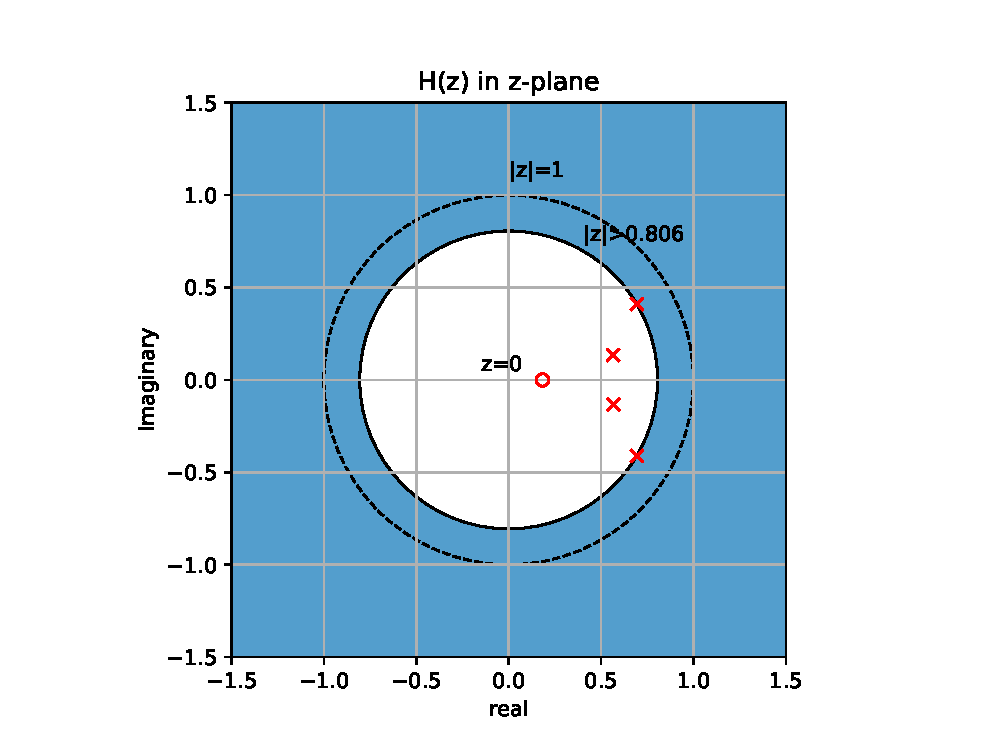
\includegraphics[width=\columnwidth]{./figs/roc}
\caption{$H(z)$ in $z$-plane}
\label{fig:xnhnfft}
\end{figure}

The code for plotting H(z) in z-plane is:
\begin{lstlisting}
codes/roc.py
\end{lstlisting}

From the figure we can observe that ROC of the system includes unit circle $\abs{z}=1$.
Which implies that the given IIR filter is stable, because h(n) is absolutely summable.

Since the audio input is bounded,and h(n) is also bounded the system is said to be stable.
\\
\textbf{Verification}:

Given bounded input - audio signal x(n) , and system difference equation \ref{eq:eqn2}

we know that the maximum value of x(n) is 0.839 and minimum value is -0.9417.

Similarly ,the maximum value of y(n) is 0.82225 and minimum value is -0.95376 and it tends to zero as n tends to infinity.

We can say that the bounded input x(n) gives bounded output
y(n). So, we can say that the system is BIBO stable i.e stable.

\item Using h(n) obtained in \ref{prob:hn} compute filtered output using the below equation of convolution
%
\begin{equation} 
\label{eq:convolution}
y(n) = x(n)*h(n) = \sum_{n=-\infty}^{\infty}x(k)h(n-k)
\end{equation}
\solution The following code plots Fig. \ref{fig:convolve}
%
\begin{lstlisting}
codes/convolve.py
\end{lstlisting}
\begin{figure}[!ht]
\centering
\includegraphics[width=\columnwidth]{./figs/convolve}
\caption{$y(n)$ from the definition of convolution}
\label{fig:convolve}
\end{figure}
The filtered sound signal through convolution from this method is found in
\begin{lstlisting}
codes/covolve_music.wav
\end{lstlisting}
We can observe that the output obtained is same as y(n) obtained in Fig. \ref{fig:plot_xy}

\end{enumerate}

\section{DFT and FFT}
\begin{enumerate}[label=\thesection.\arabic*
,ref=\thesection.\theenumi]
\item Compute
\begin{align}
        X(k) \triangleq \sum_{n=0}^{N-1} x(n) e^{-j 2 \pi k n / N}, \quad k=0,1, \ldots, N-1
\end{align}
and $H(k)$ using h(n).
\\
\solution
For this given IIR system with audio sample as x(n) and h(n) as impulse response h(n) obtained in \ref{prob:hn} 

DFT of a Input Signal $x(n)$ is 
\begin{align}
    X(k) \triangleq \sum_{n=0}^{N-1} x(n) e^{-j 2 \pi k n / N}, \quad k=0,1, \ldots, N-1
\end{align}
DFT of a Impulse Response $h(n)$ is 
\begin{align}
    H(k) \triangleq \sum_{n=0}^{N-1} h(n) e^{-j 2 \pi k n / N}, \quad k=0,1, \ldots, N-1
\end{align}

The following code plots FFT of $x(n)$ and $h(n)$ in Fig. \ref{fig:xhfft}.
\begin{lstlisting}
codes/fft_x.py
\end{lstlisting}
Magnitude and Phase plots obtained through above code is 
\begin{figure}[!ht]
\centering
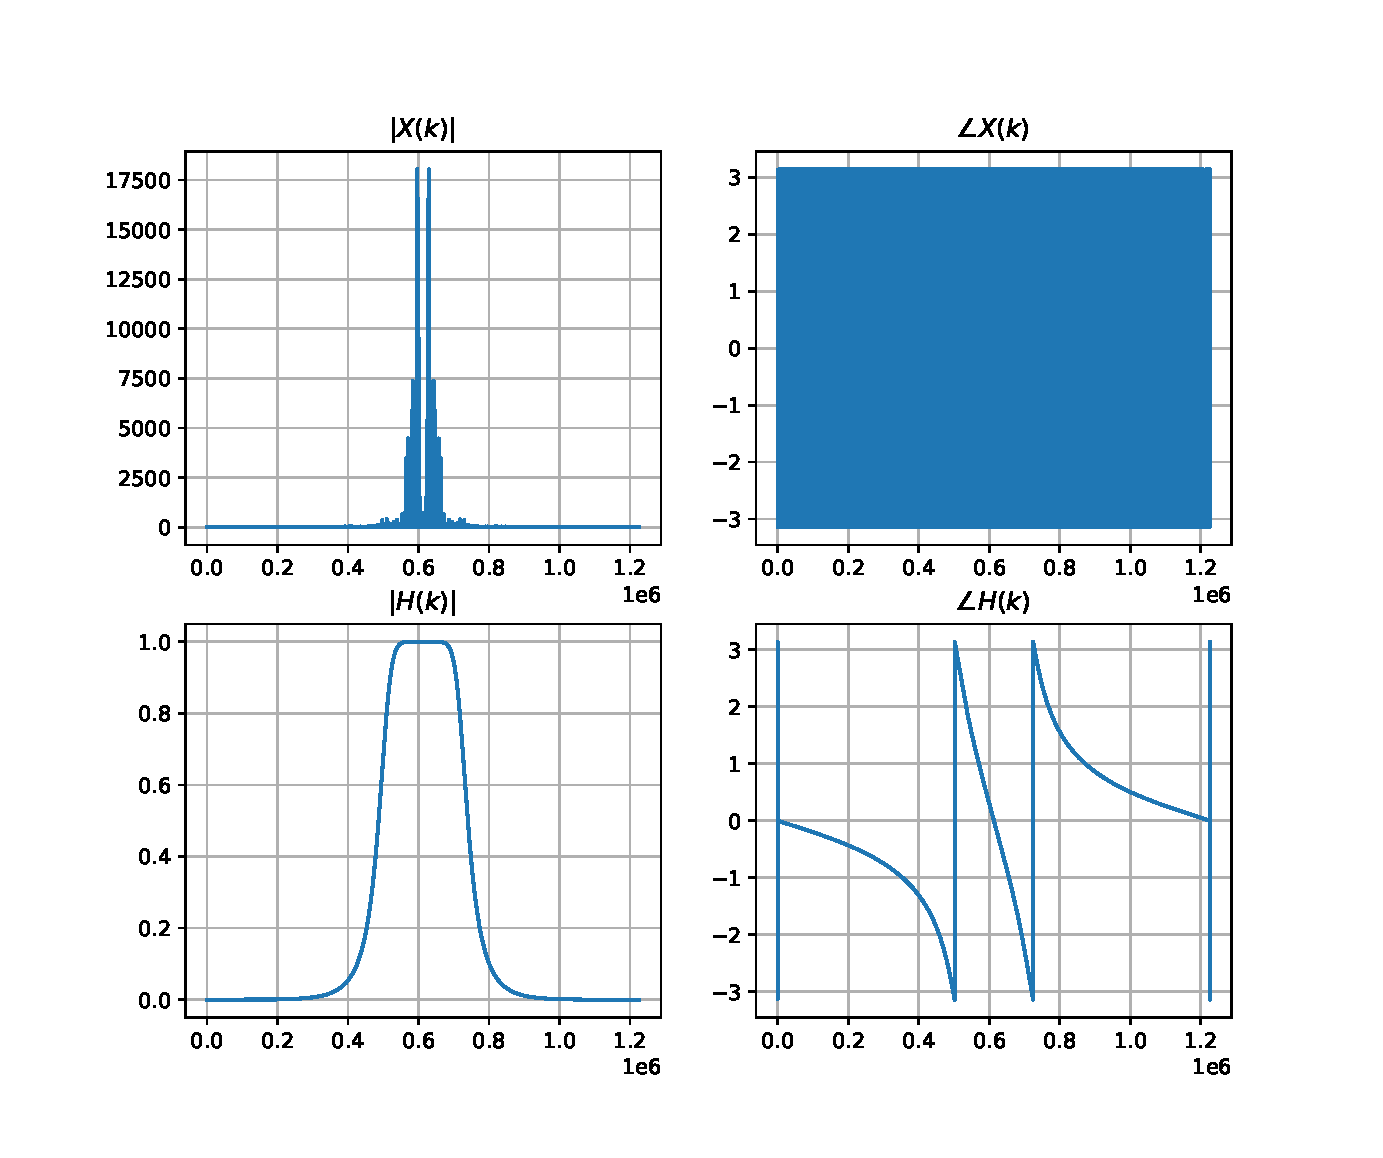
\includegraphics[width=\columnwidth]{./figs/fft_x}
\caption{$X(k)$ and $H(k)$}
\label{fig:fft_x}
\end{figure}

\item Compute
\begin{equation}
Y(k) = X(k)H(k)
\end{equation}
and using this find 
\begin{equation}
y(n) \triangleq \sum_{k=0}^{N-1} Y(k) e^{j 2 \pi k n / N}, \quad n=0,1, \ldots, N-1
\end{equation}
\\
\solution
The following code plots Fig.\ref{fig:fft_y}
\begin{lstlisting}
codes/fft_y.py
\end{lstlisting}
\begin{figure}[!ht]
\centering
\includegraphics[width=\columnwidth]{./figs/fft_y}
\caption{$y(n)$ from IFFT}
\label{fig:fft_y}
\end{figure}

The filtered sound signal from this method is found in
\begin{lstlisting}
codes/fft_music.wav
\end{lstlisting}
We can observe from the above plot that it is same as the y(n) observed in Fig.\ref{fig:plot_xy}
\end{enumerate}


\end{document}

